This report presents a solution to assignment \#2 of TDT4258 at NTNU during the spring of 2013.
The objective of this lab assignment is to write a program in C for the STK1000 development board which causes different sounds to play when different buttons on the board are pressed.
An interrupt routine should be used to pass audio samples to the board's ABDAC (Audio Bitstream Digital to Analog Converter).
The program is to run directly on the board, without an operating system.
A minimum of three different sound effects should be made, as well as a ``start up melody'' (\cite{compendium}, page 48).

The goal of this assigment is to introduce students to programming in C, I/O control for AVR32 in C, use of the microcontroller's ABDAC for sound generation and Interrupt handling in C for AVR32.

\section{The STK1000}
	The STK1000 is a development board from Atmel which offers a complete development environment for Atmel's AT32AP7000 processor.
	It offers a multitude of different peripheral I/O devices, of which this assignment will be using an array of LEDs and some push buttons, as well as the Audio Bitstream Digital-to-Analog Converter.
	The processor is an ARM32 processor, and will for this assignment be only running the assembled output of a mix of hand-coded and tool-generated C code, without the support of an operating system.

\section{The Physics and Digitalization of Sound}
	In order to write a program to generate sound, one should first study the physical properties of sound, and research different strategies to generate sound in a digital environment.

Sound is a mechanical wave that is an oscillation of pressure composed of frequencies within the range of hearing\footnote{http://en.wikipedia.org/wiki/Sound}.

Humans can percieve sounds with frequencies that range from about 20Hz - the lowest of basses - to 20kHz - the highest of high-pitched whining.
Sound is inherently analog, and requires some form of digital representation to be able to be generated by the AP7000, which is a digital device.
Regarding a sound wave as a continuous signal representing wave amplitude with respect to time, one straight-forward way of representing a sound wave digitally is to simply have an list of integer signal samples at a fixed, preferrably small, time interval.
This is indeed the format the AP7000 expects for its digital-to-analog converter.

There are different strategies available for preparing the stream of integers that needs to be sent to the digital-to-analog converter to generate a sound.
One strategy is simply to store the prepared list of integers somewhere in memory, and then copy it over to the DAC integer by integer as they are consumed by the ABDAC.
This strategy is analogous to rasterized bit maps in the image world.
This strategy, while easy to implement, and is able to represent all kinds of sounds, requires a great deal of memory (integer size * sample rate of bytes per second, in fact).
As an example, a three minute song, when stored at 16 bits per sample at a generously low sample rate of 22050Hz, requires 16 bits/sample * 180 seconds * 22050 samples/second = ̃ca 7.57 megabytes.
To put this in perspective, the entire flash memory of the AP7000 is 8 megabytes.
On a low memory platform like the STK1000, this is therefore not a great strategy.

Another strategy is the generative approach.
This strategy is analogous to vector based images in the image world.
The idea is to generate samples at run-time based on configurations read from memory, rather than reading the pre-generated values from memory.
This is a more CPU-hungry approach, but requires less memory than the previous strategy.
This strategy is used for the sound effect synth in the presented solution program.

A third strategy is a hybrid approach, where small sample lists are pre-bundled with the program, and generative rules are used to play back the samples at different times with different parameters.
This is the approach used in the music player in the presented solution program.


\section{About the MOD file format}
	The MOD file format is an old music tracker file format originally created for the Commodore Amiga (figure \ref{img-amiga}), a series of computers from the late eighties.
\begin{figure}[H]
	\caption{The Amiga 1000 (1985), the first Amiga model released. Image courtesy of Kaiiv.}
	\centering
	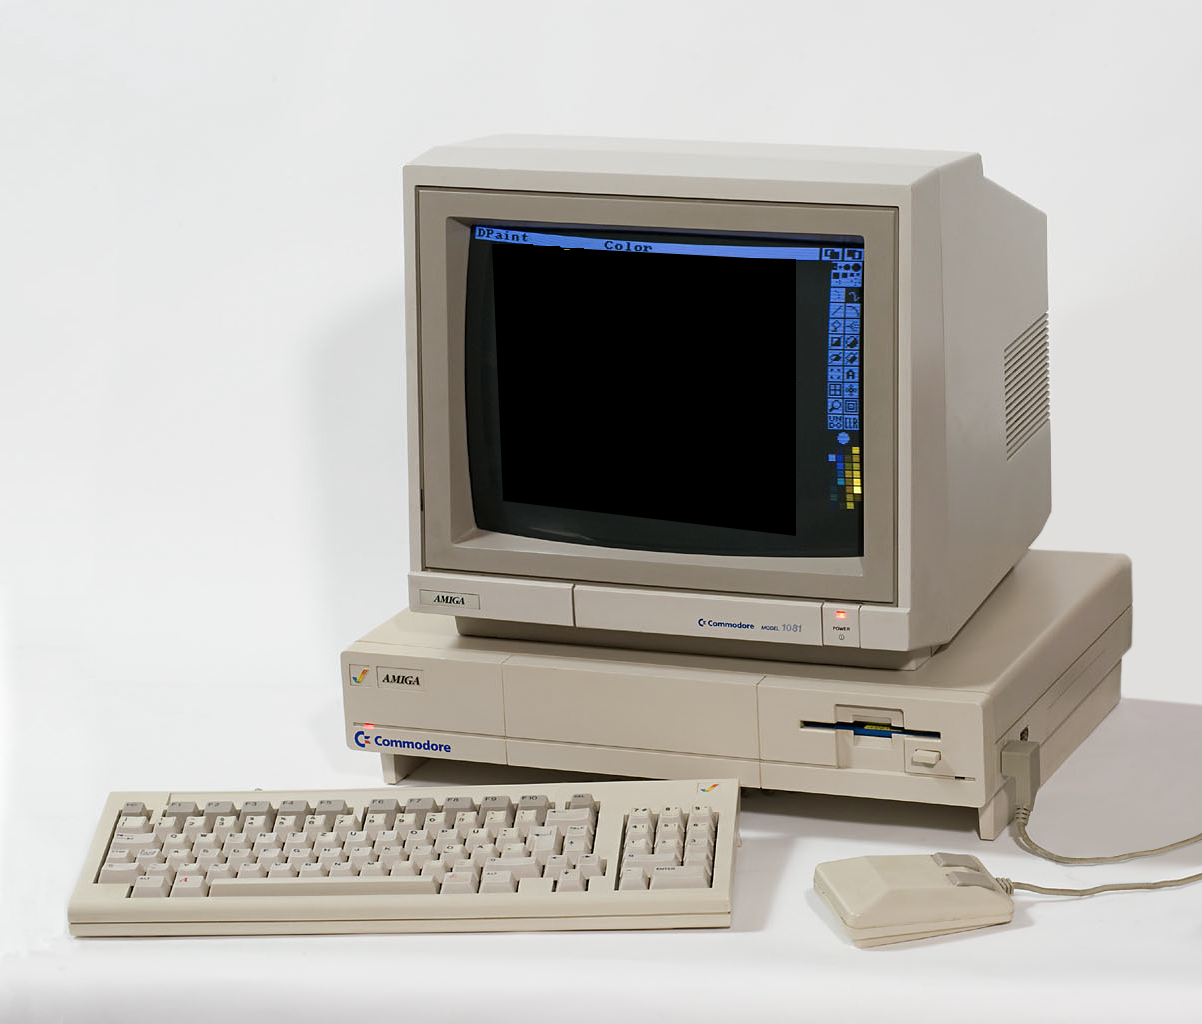
\includegraphics[width=4in]{{images/Amiga.jpg}}
    \label{img-amiga}
\end{figure}

The file format is tightly optimized for playback on the Amiga's audio hardware, so to understand the inner workings of the MOD file format, one should first know a little about how the Amiga's audio hardware works.

The Amiga's sound chip, called Paula, is capable of powering four simultaneous DMA-driven 8-bit PCM sample sound channels.
Each of these channels can be independently set to different sample frequencies many times per second.
The MOD format exploits this -- it supports 4 simultaneous channels of sample playback, using the frequency modulation to change the pitch of the samples played in the different channels.

Internally, the music in a MOD file is stored as a set of PCM-coded predefined sounds, as well as a large table of note patterns containing information about which sounds should be played at which frequencies and at which time.
The MOD format also includes a large set of musical effects such as tremolo, vibrato, arpeggio, portamento and so on, a subset of which are implemented in the presented solution program.

The MOD file format is not a defined standard, and does therefore not have a formal specification.
The MOD format grew organically from the early Amiga demoscene in the eighties, so many different variants exist -- each with with their own specialities and quirks.
The MOD Player presented in the solution is tailored to read so-called \texttt{M.K.} MODs generated by a MOD creator program (``tracker'') called ProTracker.
These MOD files are called \texttt{M.K.} MODs because they contain the magic number \texttt{M.K.} in the file header.
This is one of the most popular MOD formats, and has become a sort informal standard amongst MOD trackers.

\texttt{M.K.} MODs can have a maximum of 31 bundled PCM-coded sounds, 128 patterns, each with 64 note divisions for each of the four channels, and a a 128 item long list of which patterns should be played in what order.

Figure \ref{img-protracker} shows an image of a MOD file being edited in a tracker program.
Each column represents one channel, and each row represents one of the 64 divisions of a pattern.
The currently played division is traditionally kept vertically centered in the middle of the screen, as in this image.


\begin{figure}[H]
	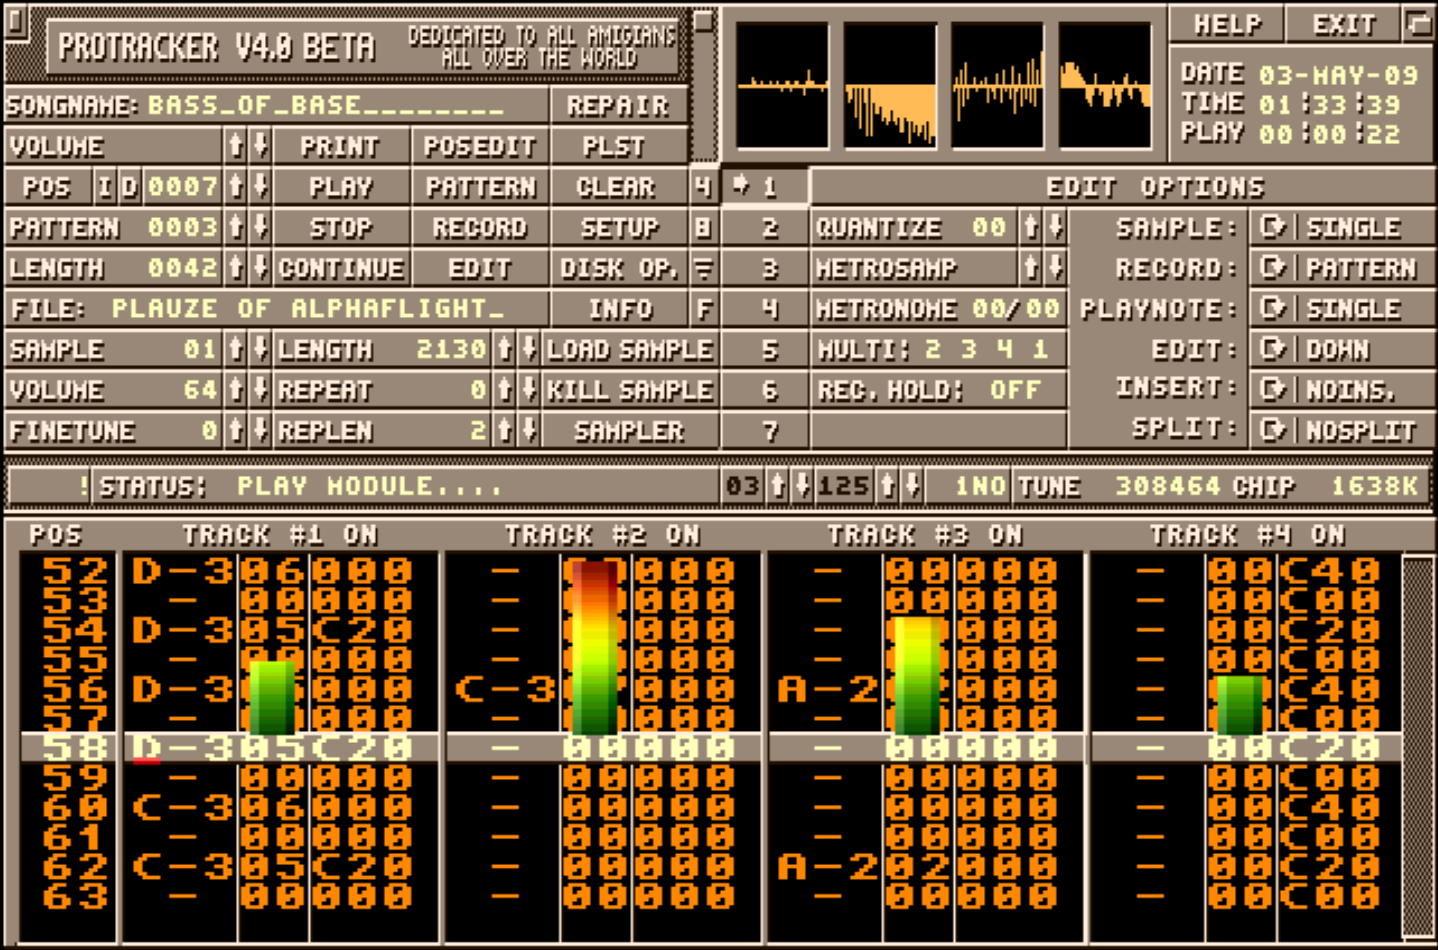
\includegraphics[width = \textwidth]{images/Protracker.png}
	\caption{A four-channel MOD being played in ProTracker. Image courtesy of Alec Graggamoor.}
	\label{img-protracker}
\end{figure}

These four resources do a pretty good job of documenting the MOD file format in detail:
\begin{itemize}
	\item{\url{http://www.mediatel.lu/workshop/audio/fileformat/h_mod.html}}
	\item{\url{http://archive.cs.uu.nl/pub/MIDI/DOC/MOD-info}}
	\item{\url{https://bel.fi/alankila/modguide/}}
	\item{\url{http://16-bits.org/mod/}}
\end{itemize}

\newpage

